\section{Summary}

\subsection{Summary}

\begin{frame}{What Have We Learned?}
    \begin{center}
        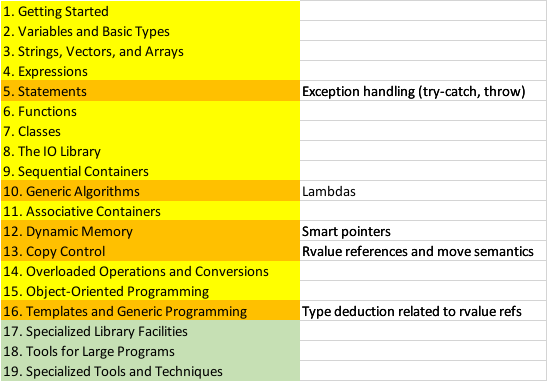
\includegraphics[width = 0.95\textwidth]{img/contents.png}
    \end{center}
\end{frame}

\begin{frame}
    \begin{center}
        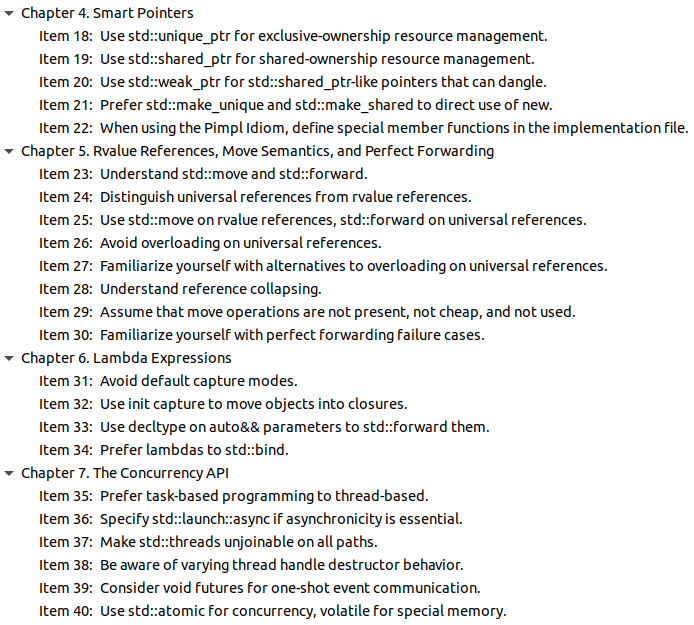
\includegraphics[width=0.85\textwidth]{img/effectivemodern.png}
    \end{center}
\end{frame}

\begin{frame}{Exception Handling}
    \begin{itemize}
        \item \ttt{try-catch}, \ttt{throw} and the exception classes defined in the standard library
        \item \textit{Effective C++} Item 8, 25, 29.
    \end{itemize}
\end{frame}

\begin{frame}{\ttt{new} and \ttt{delete}}
    \begin{itemize}
        \item Customize \ttt{new} and \ttt{delete}?
        \begin{itemize}
            \item You may want to detect usage errors, e.g. memory leak.
            \item You may have a good understanding of your program's dynamic memory usage patterns, and have a better way of allocating/deallocating memory that can improve efficiency.
            \item You may want to collect usage statistics.
            \begin{itemize}
                \item What is the distribution of allocated block sizes?
                \item What is the distribution of their lifetimes?
                \item In what order do they tend to be allocated and deallocated?
                \item What is the high water mark?
            \end{itemize}
        \end{itemize}
        \item \ttt{new} and \ttt{delete} with extra arguments?
    \end{itemize}
    \footnotesize\url{https://blog.csdn.net/qq_39677783/article/details/124704501}
\end{frame}

\begin{frame}[fragile]{Concurrency}
    Multi-threading in C++: \ttt{<thread>}, \ttt{<future>}, \dots (since C++11)
    \begin{cpp}
int calculate_sum(const int *a, int n) {
  int sum[4] = {0};
  std::vector<std::thread> th;
  int block_size = n / 4;
  for (auto i = 0; i != 4; ++i)
    th.emplace_back(
        [a](int left, int right, int &s) {
          for (auto j = left; j != right; ++j)
            s += a[j];
        }, block_size * i, block_size * (i + 1),
            std::ref(sum[i]));
  for (auto &t : th) t.join();
  for (int i = block_size * 4; i < n; ++i)
    sum[0] += a[i];
  return sum[0] + sum[1] + sum[2] + sum[3];
}
    \end{cpp}
\end{frame}

\begin{frame}[fragile]{The Boost Library}
    A collection of high quality, open source, platform- and compiler-independent libraries. \url{http://boost.org}
    \begin{itemize}
        \item Lambda: (Unlike C++11 lambda)
        \begin{cpp}
std::for_each(v.begin(), v.end(),
            std::cout << _1 * 2 + 10 << '\n');
        \end{cpp}
        \item Template metaprogramming library (mpl)
        \item Math and numerics
        \item Inter-language support (e.g. boost python)
        \item Memory management
        \item Graph library
        \item \dots\dots
    \end{itemize}
\end{frame}